% Task 4.2 report, converted from reports/task4_2_eegnet.html.
% Build: pdflatex task4_2_eegnet  (requires neurips_2024.sty next to this file
% and vector/PNG assets under figures/).
\documentclass{article}
\usepackage[preprint]{neurips_2024}

\usepackage[utf8]{inputenc}
\usepackage[T1]{fontenc}
\usepackage{lmodern}
\usepackage{graphicx}
\usepackage{booktabs}
\usepackage{amsmath,amssymb}
\usepackage{xcolor}
\usepackage[hidelinks]{hyperref}
\usepackage[section]{placeins}

\graphicspath{{figures/}}

\title{Task 4.2: A CausalEEGNet Regression Decoder for Movement Velocity
Under Amplitude-Modulated Stimulation}

\author{EECS 182 Project\\
\texttt{ianibis/EECS182-Project}\\}

\begin{document}
\maketitle

\begin{abstract}
CausalEEGNet, a modified braindecode EEGNet, predicts a macaque's index fingertip
velocity from raw local field potential (LFP: the voltage picked up by 35~electrodes
implanted over motor cortex, sampled at 1~kHz). It outputs one $(v_x, v_y)$ pair per
50~ms bin. The network is trained only on recordings made with stimulation switched
off, and tested on recordings made while it was on. On clean input the decoder reaches
a mean test $R^2$ of $+0.021$ ($+0.070$ for a five-run ensemble); on stimulated input
the same weights collapse to $-0.192$. Training with synthetic tones at the stimulator
frequency moves the stimulated score to $+0.032$ at no measurable cost on clean input.
Against the ridge baseline of task~3.1 the network is indistinguishable on clean data.
\end{abstract}

\section{Data and evaluation protocol}
\label{sec:protocol}

\begin{table}[htbp]
\centering
\caption{Split structure. One session is one continuous recording block of 50
trials, made on one day.}
\vspace{2pt}
\begin{tabular}{@{}llrl@{}}
\toprule
Stage & Sessions & Trials & Use \\
\midrule
Train      & 14 stimulation-off           & 560 & gradient updates \\
Validation & 3 stimulation-off            & 150 & early stopping and the sweep \\
Test       & 14 stimulation-on, 5 days    & --  & scored once, never trained on \\
\bottomrule
\end{tabular}
\end{table}

The 14 test sessions are scored on two inputs each: the stimulated recording itself,
and the unstimulated recording taken the same day. We call the unstimulated recording
the \emph{clean input} throughout, and no decoder was trained on either kind. Scores
are reported per day rather than per session, because the sessions from one day share
a single clean reference recording and so cannot be scored independently. The five test
days hold 1, 3, 3, 3 and 4 sessions.

\subsection{Stimulation artifacts}
\label{sec:artifact}

Stimulation delivers a 3.5~kHz carrier through the same electrodes that record LFP,
amplitude modulated at either 3~Hz or 20~Hz. The recording hardware only partly removes
the carrier, and what it leaves behind on the LFP is the artifact this task has to
survive. All five test days run at 1.75~mA: three are 3~Hz days (250520, 250609,
250613) and two are 20~Hz days (250530, 250616), and no test day mixes the two. The
frequencies were chosen by the experimenters, not by us, and enter this report only as
the frequencies we later inject as synthetic tones in Appendix~\ref{sec:tones}.

The artifact is not random noise. It restarts on every cycle of the modulation, so it
repeats every 333~ms at 3~Hz and every 50~ms at 20~Hz. The bin length is 50~ms, which
makes the two conditions behave completely differently: one bin holds exactly one 20~Hz
period, so the artifact reads as a constant offset within the bin, while one bin holds
about 6.7 periods at 3~Hz, so the artifact reads as a sawtooth inside the bin.

\begin{figure}[htbp]
\centering
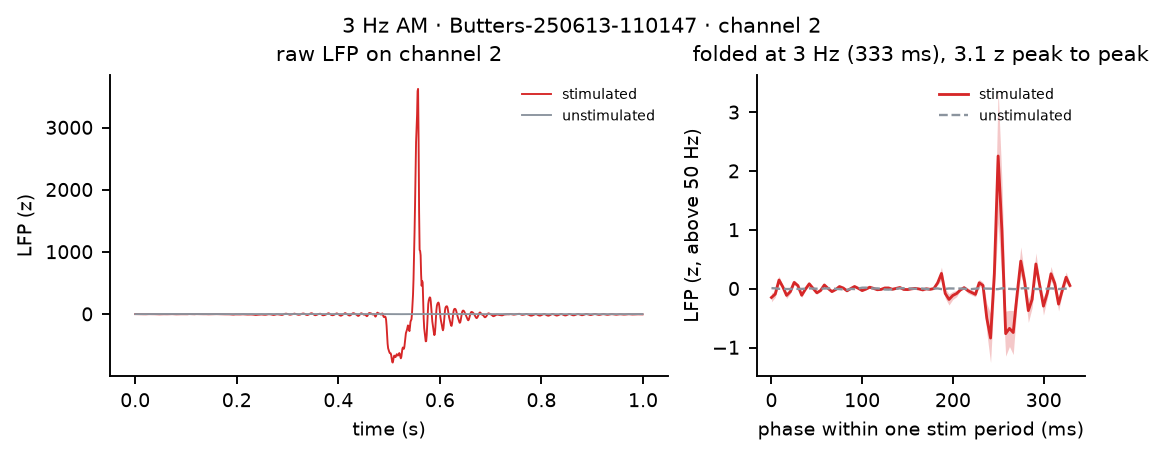
\includegraphics[width=\textwidth]{fig_artifact_3hz.png}
\caption{3~Hz day. Left: one second of raw LFP on the worst channel, stimulated against
the unstimulated recording from the same day. Right: the same recording averaged over
the stimulation period, which recovers a repeating waveform. LFP is z-scored per
channel per session.}
\label{fig:artifact3}
\end{figure}

\begin{figure}[htbp]
\centering
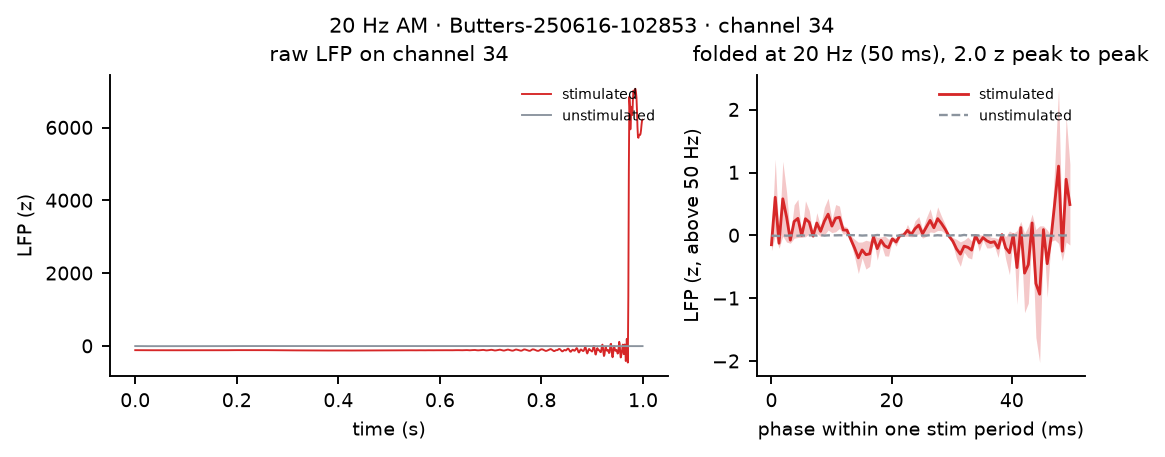
\includegraphics[width=\textwidth]{fig_artifact_20hz.png}
\caption{The same two views on a 20~Hz day. The largest transient here is a
step-and-recover rather than a clean oscillation, so the right panel is high-passed to
show the 50~ms component that survives.}
\label{fig:artifact20}
\end{figure}

Average the recording across cycles at a fixed position in the cycle, and the artifact
appears as one waveform while everything else cancels. Table~\ref{tab:artifact} measures
that waveform. On the worst channel it is 3.1~z at 3~Hz and 2.0~z at 20~Hz. The median
channel averages to 0.05~z and 0.04~z, and the unstimulated recording from the same day
averages flat at 0.04~z and 0.02~z. All LFP in this report is z-scored per channel per
session, so 1~z is one robust standard deviation of that channel's own signal.

\begin{table}[htbp]
\centering
\caption{Cycle-averaged artifact per modulation frequency, in z units.}
\vspace{2pt}
\small
\begin{tabular}{@{}llccccc@{}}
\toprule
Modul. & Period & Worst ch. & Cycle-avg. & Cycle-avg. & Cycle-avg. & Largest single \\
       &        &           & worst ch.  & median ch. & clean input & transient \\
\midrule
3 Hz   & 333 ms & 2  & 3.1~z  & 0.05~z & 0.04~z & 3622~z \\
20 Hz  & 50 ms  & 34 & 2.0~z  & 0.04~z & 0.02~z & 7064~z \\
\bottomrule
\end{tabular}
\label{tab:artifact}
\end{table}

Two properties of the artifact follow. It sits on one or two electrodes, which is why
task~3 clips z-scored features at $\pm10$ so a single bin cannot dominate the weights.
And it dwarfs the neural signal underneath it: single transients reach 3622~z and
7064~z, which is 143 and 279 times the largest excursion anywhere in the same channel's
unstimulated recording (25~z).

\section{Model architecture (4.2.1)}
\label{sec:arch}

The decoder is braindecode's \texttt{EEGNet}, a small convolutional network built for
one label per window. Its convolutions pad symmetrically and its head pools the time
axis away, so it needs two changes before it can regress one velocity pair per 50~ms
bin:
\begin{itemize}
\item \texttt{final\_conv\_length=1} and \texttt{n\_outputs=2} keep one velocity pair
per time step. Pooling 2 then 25 maps 2{,}000 samples to 40 bins of 50~ms.
\item Every padded temporal convolution is rebuilt as an explicit left-only
\texttt{ConstantPad2d} plus an unpadded convolution, so bin $t$ depends only on samples
$\le t$.
\end{itemize}

\begin{figure}[htbp]
\centering
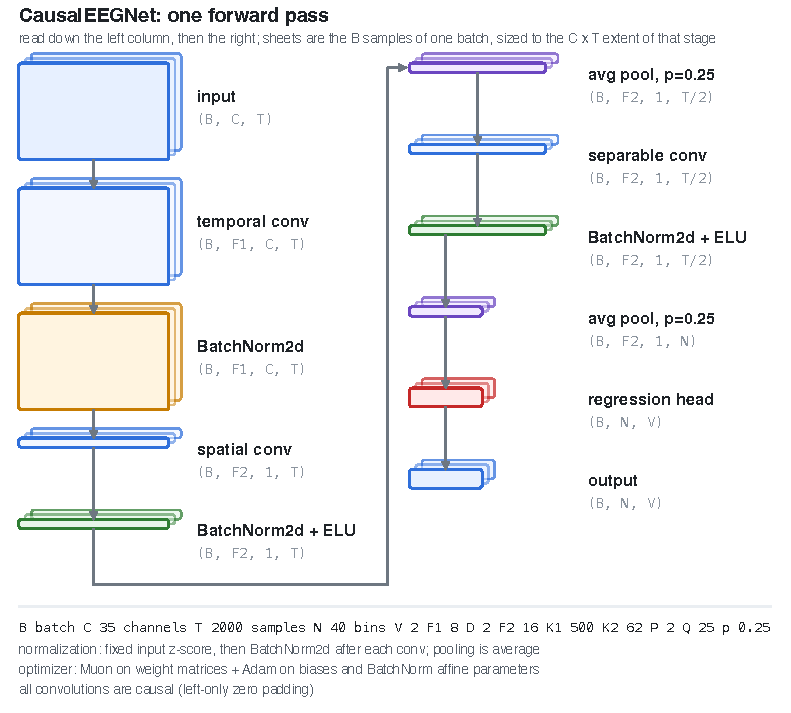
\includegraphics[width=0.62\textwidth]{eegnet_block_diagram.pdf}
\caption{One forward pass, read in two columns left to right. The stacked rectangles
are the $B$ samples of a single batch, and each sheet is drawn at the spatial extent of
that stage; the grey annotation at the top right of each graphic is its symbolic tensor
shape, in the variables listed under the diagram.}
\label{fig:arch}
\end{figure}

The spatial block is a \texttt{ParametrizedConv2dWithConstraint}, and in every saved
model all 16 spatial filters sit at L2 norm exactly 1.000: the max-norm constraint is
binding, so only the direction of each spatial filter is learned, never its scale.

\section{Hyperparameter sweep and selected setting (4.2.2)}
\label{sec:sweep}

Three knobs matter here: the temporal kernel length (how many milliseconds of LFP one
filter sees), the depth multiplier (how many spatial filters the separable block builds)
and the dropout rate. Eight configurations were trained: braindecode's defaults, five
single-knob changes from the defaults, and two changes at once. Each was trained once
and ranked by validation $R^2$, the $R^2$ it reached on the 150 held-out trials at its
best epoch. An epoch is one full pass over the 560 training trials.

\begin{table}[htbp]
\centering
\caption{Sweep results, ranked by validation $R^2$.}
\vspace{2pt}
\begin{tabular}{@{}lcccccc@{}}
\toprule
Kernel & Depth mult. & Dropout & Validation $R^2$ & Best epoch & Last epoch run \\
\midrule
500 ms  & 2 & 0.25 & $+0.1463$ & 48  & 68 \\
250 ms  & 2 & 0.5  & $+0.1378$ & 108 & 128 \\
500 ms  & 2 & 0.5  & $+0.1351$ & 56  & 76 \\
250 ms  & 2 & 0.25 & $+0.1293$ & 70  & 90 \\
500 ms  & 2 & 0.75 & $+0.1155$ & 38  & 58 \\
1000 ms & 2 & 0.5  & $+0.1149$ & 56  & 76 \\
500 ms  & 1 & 0.5  & $+0.0943$ & 48  & 68 \\
1000 ms & 2 & 0.25 & $+0.0908$ & 11  & 31 \\
\bottomrule
\end{tabular}
\label{tab:sweep}
\end{table}

The winner is the 500~ms kernel at dropout 0.25, the same kernel as the default setting
with the dropout halved. Its margin over the default ($+0.1351$) is $+0.0112$, which
equals the standard deviation across five repeated training runs at the chosen setting
(Section~\ref{sec:seeds}). A sweep cannot resolve a gap that size, so the honest reading
is that dropout 0.25 and 0.5 perform the same at this training budget. The 1000~ms kernel
at dropout 0.25 stopped improving at epoch 11, the earliest collapse of the eight.

\section{Five training runs and what a seed controls (4.2.3)}
\label{sec:seeds}

``Five seeds'' means five independent runs of the same CausalEEGNet on the same 560
stimulation-off trials. Nothing about the data, the architecture or the code changes
between them. Only the random numbers drawn during training change, and a \emph{seed} is
the integer that fixes which numbers a run draws. Five seeds give five versions of one
method. Except where a table says otherwise, every method score reported after this
section is a summary across those five runs. The 8-configuration sweep in
Section~\ref{sec:sweep} is the exception: each configuration there was trained once.

The 560 training trials sit in one array, concatenated from the 14 stimulation-off
sessions in split order, 40 trials per session. The velocity targets, the mask marking
trials whose kinematics are missing, and the 150 held-out validation trials are the same
array in every run.

One training run of CausalEEGNet proceeds as follows, and the seed selects the random
numbers at three points inside it (Figure~\ref{fig:sampling}):
\begin{enumerate}
\item \textbf{Weight initialisation.} The network's 6{,}005 weights are drawn at random
before training starts, so two runs with the same seed begin from the same starting
weights. In the runs reported here this was not actually controlled; see the note in
Section~\ref{sec:caveats}.
\item \textbf{Batch order.} At the start of each epoch the seed draws a new random
ordering of the 560 trial indices. Trials are then taken 16 at a time from that ordering,
giving 35 batches and 35 gradient steps per epoch. Batch $i$ therefore holds different
trials in different epochs and different runs; only the array itself is fixed.
\item \textbf{Dropout.} During each forward pass, dropout switches off a random 25\,\%
of units, the rate selected in Section~\ref{sec:sweep}. The seed fixes which units.
\end{enumerate}

\begin{figure}[htbp]
\centering
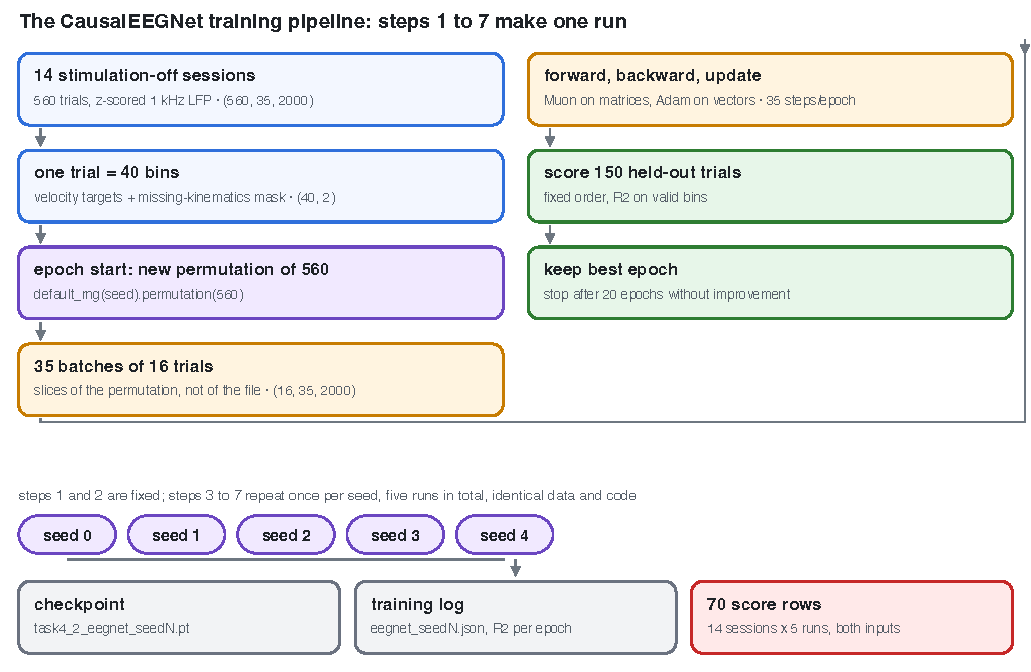
\includegraphics[width=0.72\textwidth]{eegnet_sampling.pdf}
\caption{How the trials are stored, ordered and scored. The grey annotation on the right
of each block is an array shape: 560 trials of 35 channels $\times$ 2{,}000 samples; 40
velocity bins per trial; 16 trials per batch.}
\label{fig:sampling}
\end{figure}

A run is that loop, repeated for up to 200 epochs. After each epoch we score the model
on the 150 held-out trials, keep the weights of the best-scoring epoch, and stop early if
20 epochs pass with no improvement. Each run writes one checkpoint,
\texttt{task4\_2\_eegnet\_seedN.pt} with its 6{,}005 weights, and one log with the
training loss and validation $R^2$ of every epoch. No test data is used at any point in
that loop.

\subsection*{What is optimised, and what R\textsuperscript{2} measures}
Each run minimises the mean squared error over velocity bins whose kinematics are valid:
\begin{equation}
L = \frac{1}{M} \sum_{b \in \mathrm{valid}} \lVert \hat{\mathbf{v}}_b - \mathbf{v}_b \rVert^2 ,
\end{equation}
with $\mathbf{v}_b$ the measured $(v_x, v_y)$ pair of bin $b$, $\hat{\mathbf{v}}_b$ the
prediction, and $M$ the number of valid bins. Reported scores are per-axis $R^2$ averaged
over the two axes:
\begin{equation}
R^2_{\mathrm{axis}} = 1 - \frac{SS_{\mathrm{res}}}{SS_{\mathrm{tot}}}
= 1 - \frac{\sum_b (y_b - \hat{y}_b)^2}{\sum_b (y_b - \bar{y})^2},
\qquad
R^2 = \tfrac{1}{2}\left(R^2_{v_x} + R^2_{v_y}\right),
\end{equation}
where $y$ is one axis of the measured velocity, $\hat{y}$ its prediction and $\bar{y}$ the
mean over the scored bins. $R^2 = 1$ is exact, $R^2 = 0$ equals predicting $\bar{y}$, and
$R^2 < 0$ is worse than that constant. $SS_{\mathrm{tot}}$ is the recording's own variance,
which is what makes $R^2$ unit-free and comparable across days.

We ran the loop five times, with seeds 0 to 4, and got best validation $R^2$ of 0.146,
0.140, 0.122, 0.145, 0.125. Their mean is 0.136 and their standard deviation is 0.011.
Since data, architecture and code are identical across the five, that 0.011 is the cost
of the random numbers alone: it is how far this method's score moves depending only on
which seed drew which numbers. It sets the resolution of every comparison in this report.
A gap between two methods under about 0.01 $R^2$ cannot be told apart from luck of the
draw.

How the five runs become one number differs by table. The per-day rows in
Sections~\ref{sec:results} and~\ref{sec:ridge} and the per-day table are the arithmetic
mean of the five runs' scores. The ensemble row of Section~\ref{sec:ensemble} averages
the five runs' predictions bin by bin and scores that single averaged prediction once.
Figure~\ref{fig:curves} is not averaged either: it plots the five runs individually,
during training and at their final scores.

\begin{figure}[htbp]
\centering
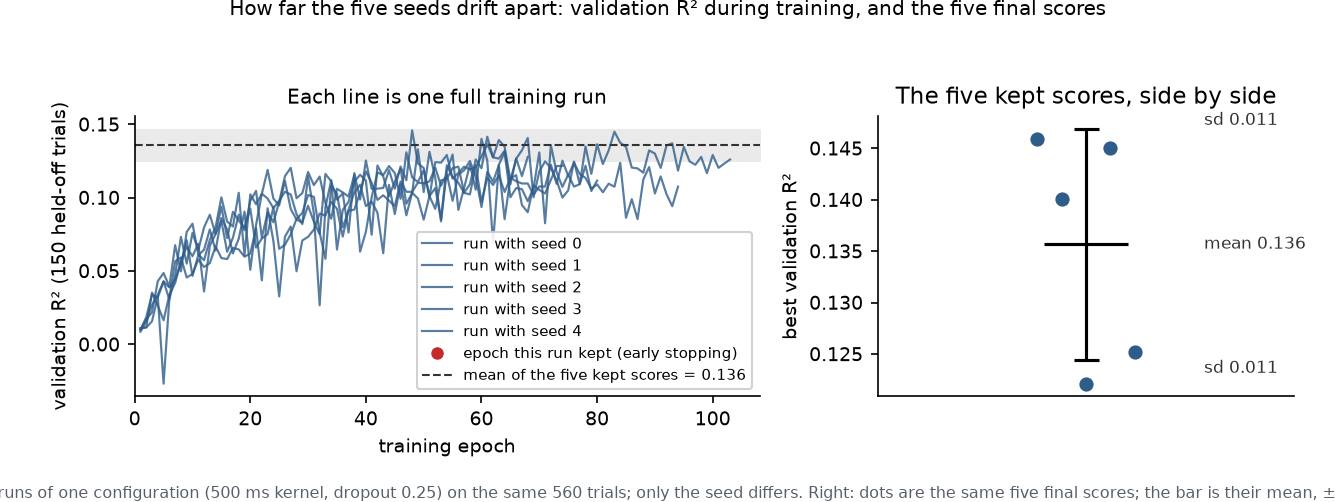
\includegraphics[width=\textwidth]{fig_val_curves.png}
\caption{Left: validation $R^2$ of each of the five runs after every training epoch. A run
keeps fluctuating because its data and parameters change at each step; the red dot marks the
epoch early stopping selected, and only that epoch's weights are kept. Right: the five kept
scores with their mean and $\pm 1$ sd, the 0.011 that sets this report's resolution.}
\label{fig:curves}
\end{figure}

\begin{table}[htbp]
\centering
\caption{Per-run validation results for the five baseline runs.}
\vspace{2pt}
\begin{tabular}{@{}lccc@{}}
\toprule
Seed & Best validation $R^2$ & Best epoch & Last epoch run \\
\midrule
0 & $+0.146$ & 48 & 68 \\
1 & $+0.140$ & 60 & 80 \\
2 & $+0.122$ & 54 & 74 \\
3 & $+0.145$ & 83 & 103 \\
4 & $+0.125$ & 74 & 94 \\
\bottomrule
\end{tabular}
\label{tab:seeds}
\end{table}

Over the five runs, baseline training averages $0.1357 \pm 0.0112$ on validation.

\section{Test scores: unstimulated input versus stimulated input (4.2.4)}
\label{sec:results}

\begin{figure}[htbp]
\centering
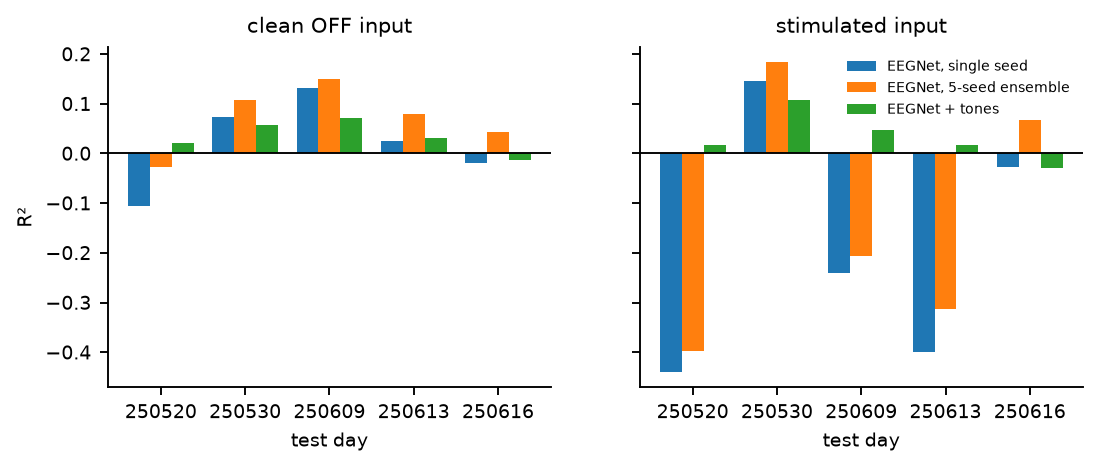
\includegraphics[width=\textwidth]{fig_perday_r2.png}
\caption{Per-day $R^2$ on clean input (left) and stimulated input (right).}
\label{fig:perday}
\end{figure}

\begin{table}[htbp]
\centering
\caption{Test $R^2$ by decoder and input type, with bootstrap 95\% CIs over the five days.
The tone row is Appendix~\ref{sec:tones}.}
\vspace{2pt}
\small
\begin{tabular}{@{}lcc@{}}
\toprule
Decoder & Clean input, $R^2$ [95\% CI] & Stimulated input, $R^2$ [95\% CI] \\
\midrule
EEGNet, baseline (mean of 5 runs)   & $+0.021\ [-0.053, +0.087]$ & $-0.192\ [-0.383, -0.001]$ \\
EEGNet, ensemble of 5 runs          & $+0.070\ [+0.013, +0.118]$ & $-0.134\ [-0.326, +0.059]$ \\
EEGNet + tones (see App.~A)      & $+0.033\ [+0.008, +0.058]$ & $+0.032\ [-0.005, +0.072]$ \\
\bottomrule
\end{tabular}
\label{tab:main}
\end{table}

Each entry of Table~\ref{tab:main} is the mean over the five days, and the interval is a
bootstrap 95\% confidence interval resampled over those five days. So the interval
reflects day-to-day variation, and with only five days it is wide.

The baseline decoder scores $+0.021$ on clean input and $-0.192$ on stimulated input, so
those weights do not survive the stimulator being switched on. Its clean-input score is the
mean of the five runs of Section~\ref{sec:seeds}.

The main result of task~4.2 is the third row: the same network, trained with synthetic tones
injected into its training trials, holds steady across both inputs ($+0.033$ clean, $+0.032$
stimulated). It beats the baseline on stimulated input by $+0.225$ $R^2$ (95\% CI $+0.049$ to
$+0.407$), scores higher on 3 of the 5 days, and costs $+0.012$ on clean input (95\% CI
$-0.035$ to $+0.078$), no measurable loss. The augmentation itself is Appendix~\ref{sec:tones},
which defines it and argues what it does and does not show; the number is reported here because
it is the headline.

\subsection{Reading R\textsuperscript{2} as a velocity error in cm/s}
\label{sec:r2}

The formulas are in Section~\ref{sec:seeds}. Because $R^2$ divides by each recording's own
variance it is unit-free: a day with large movements can score well while making large
absolute errors, and a quiet day can score badly while making small ones. RMSE is the view
that keeps units, and it says how much that matters in cm/s.

RMSE is the view that keeps units. Per bin we take the 2-D velocity error
$e = \sqrt{e_{v_x}^2 + e_{v_y}^2}$ in cm/s, and RMSE is its root mean square over all
bins. Predicting the mean velocity gives an expected RMSE of $\sqrt{2} \times
\mathrm{sd}(\mathrm{speed})$. On these five days the index fingertip moves with a
standard deviation of 43--48~cm/s per axis, so the mean predictor sits at
61--68~cm/s. Any decoder worth having must beat that.

\begin{figure}[htbp]
\centering
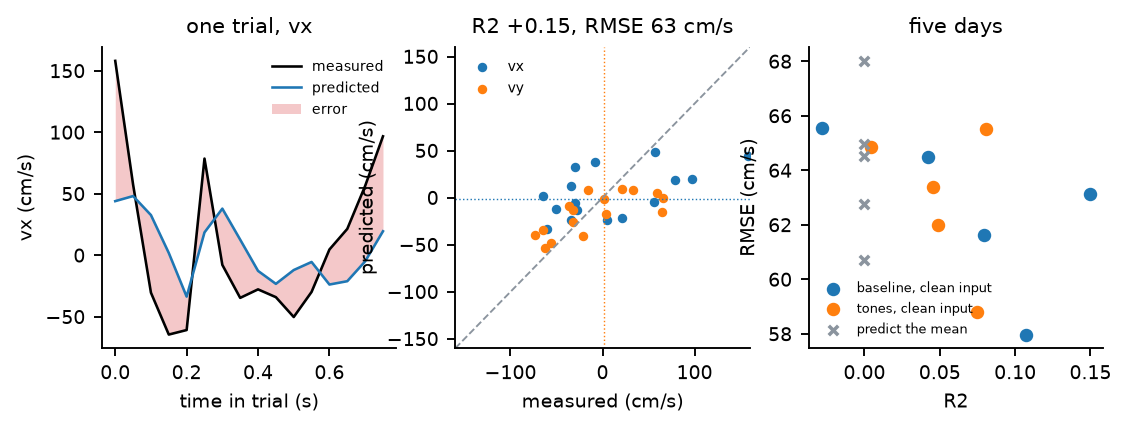
\includegraphics[width=\textwidth]{fig_r2_vs_rmse.png}
\caption{Left: one trial from the clean recording of day 250609, measured against
predicted $v_x$; the shaded band is the error $R^2$ penalises. Middle: predicted against
measured for both axes. The cloud is flatter than the dashed identity line, so the
decoder under-predicts large velocities; that shrinkage toward zero is what a low $R^2$
measures. Dotted lines mark the mean predictor. Right: $R^2$ against RMSE for the five
days, with the mean predictor's error as grey crosses.}
\label{fig:r2rmse}
\end{figure}

\begin{table}[htbp]
\centering
\caption{Per-day velocity error on clean input.}
\vspace{2pt}
\small
\begin{tabular}{@{}lcccccc@{}}
\toprule
Day & Speed sd & Mean-pred. & Ensemble & Ensemble & Tones & Tones \\
    & (cm/s) & RMSE (cm/s) & $R^2$ & RMSE (cm/s) & $R^2$ & RMSE (cm/s) \\
\midrule
250520 & 46 & 65 & $-0.028$ & 65.6 & $+0.045$ & 63.4 \\
250530 & 43 & 61 & $+0.107$ & 58.0 & $+0.075$ & 58.8 \\
250609 & 48 & 68 & $+0.150$ & 63.2 & $+0.080$ & 65.5 \\
250613 & 44 & 63 & $+0.079$ & 61.6 & $+0.049$ & 62.0 \\
250616 & 46 & 65 & $+0.042$ & 64.5 & $+0.004$ & 64.9 \\
\bottomrule
\end{tabular}
\label{tab:error}
\end{table}

Every $R^2$ and RMSE in Table~\ref{tab:error} comes from the ensemble prediction, the
five-run average of predictions described in Section~\ref{sec:ensemble}, so these columns
match the ensemble row of Table~\ref{tab:main} and not any single run.

$R^2$ and RMSE agree about which days decode well and disagree about how good that is. On
day 250609 the ensemble reaches $v_x$ $R^2$ $+0.06$ and $v_y$ $R^2$ $+0.24$, and its RMSE
of 63.2~cm/s beats the mean predictor's 68.0~cm/s by 7\,\%. Averaged over the five days
the ensemble's $+0.070$ corresponds to a 3\,\% error reduction. ``$R^2$ 0.15'' sounds
much better than ``7\,\% less velocity error'' for the same predictions, which is why
this table quotes both.

\section{Ensemble: averaging the five models' predictions (4.2.5)}
\label{sec:ensemble}

\begin{figure}[htbp]
\centering
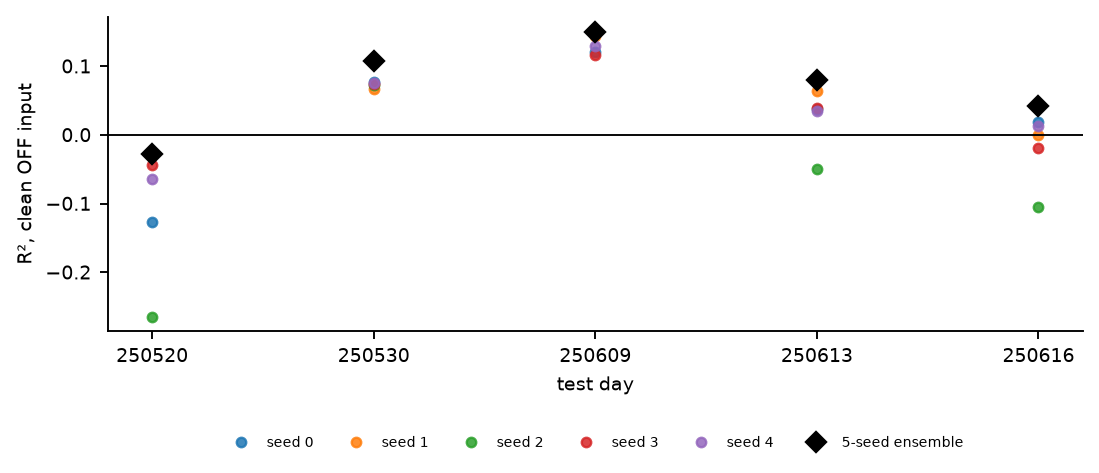
\includegraphics[width=\textwidth]{fig_ensemble.png}
\caption{Clean-input $R^2$ for each of the five runs and for the ensemble, on the same
input.}
\label{fig:ensemble}
\end{figure}

The scores in Sections~\ref{sec:results} and~\ref{sec:ridge} average five numbers: each
run's score, then their mean. This section averages five models. We load all five
checkpoints, run each on the same input, average their predicted $(v_x, v_y)$ pairs bin
by bin, and compute $R^2$ once from that averaged prediction. It is a different decoder,
not a different way of reporting.

The two differ because the five runs make partly independent mistakes. Averaging their
outputs cancels some of that error before the metric is computed, which averaging five
$R^2$ values cannot do. The gain appears where it should: clean-input $R^2$ rises from
$+0.021$ (mean of five separate scores) to $+0.070$ (one score from averaged
predictions), and the gain is largest on the days where the five runs disagree most. Day
250520 gains $+0.077$ against a five-run spread of 0.097; day 250616 gains $+0.061$
against a spread of 0.050.

The ensemble costs five forward passes at inference and has no single weight file. It is
stored in the results with \texttt{seed = -1} so that grouping by seed does not mistake
it for a sixth run of seed 0.

\section{EEGNet compared with the ridge baseline (4.2.6)}
\label{sec:ridge}

The reference decoder is the ridge regression from task~3.1, and its scores come from
that task's output file rather than anything trained here. It is a linear model on
engineered features, not on raw LFP: per 50~ms bin it takes the local motor potential
(LMP, a causal 256~ms moving average of the LFP) and seven band-power features from each
of the 35 electrodes, appends nine earlier bins of that history, and fits ridge
regression to the same velocity targets. It is trained on the same 14 stimulation-off
sessions and scored on the same clean input, so the comparison with EEGNet is
like-for-like on data and metric. It also costs nothing to train: no epochs, no seed, no
dropout.

Across the five days EEGNet scores $-0.024$ $R^2$ below ridge (mean of eegnet $-$ ridge;
95\% CI $-0.119$ to $+0.047$) and wins on 2 of 5 days. One day carries the whole
deficit: 250520 has a single test session, and there EEGNet scores $-0.106$ against
ridge's $+0.084$. Drop that day and EEGNet is $+0.017$ ahead. On clean input the two
decoders are indistinguishable at five days, and the convolutional network earns nothing
for its 200-epoch budget over a linear model on hand-built features.

\begin{table}[htbp]
\centering
\caption{Per-day test $R^2$ for every decoder and input. Columns 2--5 are clean input;
the last two are stimulated input. ``Run spread'' is the standard deviation of the five
baseline runs.}
\vspace{2pt}
\small
\begin{tabular}{@{}lccccccc@{}}
\toprule
Day & Ridge (3.1) & EEGNet & Run spread & Ensemble & + tones & Baseline & Tones \\
    &             & clean  & (sd)       & clean    & clean   & stim.    & stim. \\
\midrule
250520 & $+0.084$ & $-0.106$ & 0.097 & $-0.028$ & $+0.022$ & $-0.439$ & $+0.018$ \\
250530 & $+0.037$ & $+0.073$ & 0.004 & $+0.107$ & $+0.058$ & $+0.145$ & $+0.108$ \\
250609 & $+0.046$ & $+0.132$ & 0.014 & $+0.150$ & $+0.071$ & $-0.240$ & $+0.048$ \\
250613 & $+0.038$ & $+0.025$ & 0.043 & $+0.079$ & $+0.030$ & $-0.399$ & $+0.017$ \\
250616 & $+0.022$ & $-0.019$ & 0.050 & $+0.042$ & $-0.014$ & $-0.027$ & $-0.030$ \\
\bottomrule
\end{tabular}
\label{tab:perday}
\end{table}

\section{Checkpoints (4.2.7)}
\label{sec:ckpt}

Ten \texttt{state\_dict} files of 31~KB each, one per run per method, holding 21 tensors
and 6{,}005 parameters. All ten load strictly into the notebook class. Loading each one
and rescoring the validation days reproduces the logged \texttt{best\_val\_r2} to 1e-5,
and rescoring the 14 test sessions reproduces all 154 rows of
\texttt{task4\_2\_eegnet\_off.csv} exactly. The files are inference-only artifacts: they
hold no optimiser state and no hyperparameters, and their keys are positional
(\texttt{layers.3}, \texttt{layers.11}, \dots). A change to layer order therefore fails
loudly at load instead of silently mis-wiring the weights.

\begin{table}[htbp]
\centering
\caption{Checkpoint inventory. Each file holds 21 tensors and 6{,}005 parameters, loads
strictly, and is 31~KB.}
\vspace{2pt}
\begin{tabular}{@{}llc@{}}
\toprule
File & Validation $R^2$ & Load \\
\midrule
\texttt{task4\_2\_eegnet\_seed0.pt}                     & $+0.146$ & ok \\
\texttt{task4\_2\_eegnet\_seed1.pt}                     & $+0.140$ & ok \\
\texttt{task4\_2\_eegnet\_seed2.pt}                     & $+0.122$ & ok \\
\texttt{task4\_2\_eegnet\_seed3.pt}                     & $+0.145$ & ok \\
\texttt{task4\_2\_eegnet\_seed4.pt}                     & $+0.125$ & ok \\
\texttt{task4\_2\_eegnet\_stimulation\_tones\_seed0.pt} & $+0.064$ & ok \\
\texttt{task4\_2\_eegnet\_stimulation\_tones\_seed1.pt} & $+0.070$ & ok \\
\texttt{task4\_2\_eegnet\_stimulation\_tones\_seed2.pt} & $+0.072$ & ok \\
\texttt{task4\_2\_eegnet\_stimulation\_tones\_seed3.pt} & $+0.072$ & ok \\
\texttt{task4\_2\_eegnet\_stimulation\_tones\_seed4.pt} & $+0.058$ & ok \\
\bottomrule
\end{tabular}
\label{tab:ckpt}
\end{table}

\section{Appendix A: Synthetic tone augmentation}
\label{sec:tones}

This appendix is separate because the augmentation is a design choice, not part of the
baseline evaluation. Everything in Sections~\ref{sec:arch} to~\ref{sec:ckpt} is the plain
CausalEEGNet; only the row marked ``synthetic tones'' used what follows. The baseline
decoder never sees stimulation, so its stimulated-input score measures transfer to novel
data rather than decoding skill. Adding periodic interference to the training trials is the
cheapest way to narrow that gap without touching a single label: we superimpose a sine at
the stimulator frequency on every training trial.

\begin{table}[htbp]
\centering
\caption{The tone augmentation.}
\vspace{2pt}
\small
\begin{tabular}{@{}llclc@{}}
\toprule
Augmentation & Tone freq. & Period & Bins/period & What is added \\
\midrule
tone at 3 Hz condition  & 3 Hz  & 333 ms & 6.7 & one sine per trial, random \\
tone at 20 Hz condition & 20 Hz & 50 ms  & 1.0 & phase, amplitude 0.5--3 z, \\
                        &       &        &     & per-channel gain 0.5--1.5 z \\
\bottomrule
\end{tabular}
\label{tab:tones}
\end{table}

The tone frequencies are the ones the experiment used (2.99--19.90~Hz measured), so the
3~Hz and 20~Hz test days each face a matching tone in training. The augmentation touches
only the training set, no target changes, nothing is fitted to a test session, and each
test day is still scored once.

The amplitude range is in z units, because the LFP is z-scored per channel per session
against its own median and median absolute deviation (MAD). A 0.5--3~z tone is therefore
half a standard deviation to three standard deviations of that channel's own signal,
which matches the size of the artifact's cycle-locked component measured in
Section~\ref{sec:artifact} (3.1~z and 2.0~z peak to peak on the worst channel). We did
not try to match the peak transients, which are three orders of magnitude larger and
would saturate the network.

\begin{figure}[htbp]
\centering
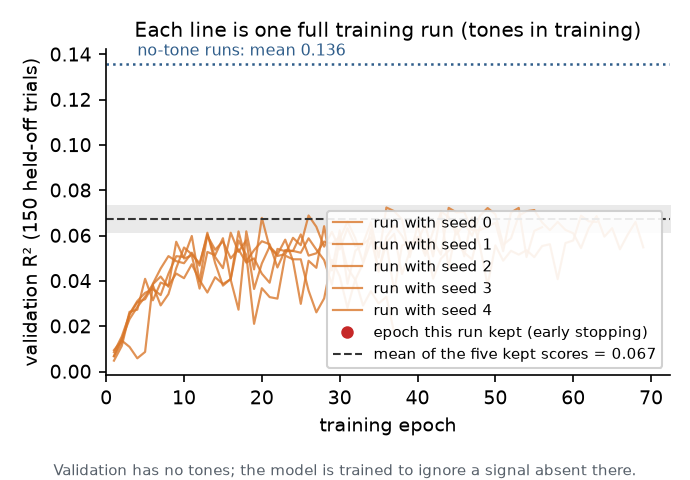
\includegraphics[width=0.6\textwidth]{fig_tones_curves.png}
\caption{Validation $R^2$ after every training epoch for the five tone-augmented runs. The
dotted line is the no-tone runs' mean of 0.136 from Section~\ref{sec:seeds}. Both groups are
scored on clean validation trials; only the tone runs have sines injected, and only during
training.}
\label{fig:tonescurves}
\end{figure}

\begin{table}[htbp]
\centering
\caption{Per-run validation results for the five tone-augmented runs.}
\vspace{2pt}
\begin{tabular}{@{}lccc@{}}
\toprule
Seed & Best validation $R^2$ & Best epoch & Last epoch run \\
\midrule
0 & $+0.064$ & 28 & 48 \\
1 & $+0.070$ & 43 & 63 \\
2 & $+0.072$ & 49 & 69 \\
3 & $+0.072$ & 36 & 56 \\
4 & $+0.058$ & 17 & 37 \\
\bottomrule
\end{tabular}
\label{tab:tonesruns}
\end{table}

The tone runs reach $0.0673 \pm 0.0063$ on validation against the no-tone runs'
$0.1357 \pm 0.0112$. The trade is a loss of clean-input accuracy against a gain on
stimulated input.
Validation $R^2$ falls from 0.136 to 0.067, since the model is asked to ignore a
component absent from clean data. In the stimulated column of Section~\ref{sec:results},
the same five runs go from $-0.192$ to $+0.032$ $R^2$. A sine is a rough stand-in for the
real artifact, which is a step-and-recover transient, so this result supports a narrow
reading: periodic interference at the stimulator frequency is the damaging part of the
artifact. It does not make the tone model a matched artifact model.

\section{Caveats}
\label{sec:caveats}

\begin{quote}
The reported runs did not seed the weight initialisation:
\texttt{torch.manual\_seed} was called after the model was constructed, so the starting
weights came from whatever the global RNG held at that moment, which in a full notebook
run is the residue of the previous training call. Seed then controlled batch order and
dropout only. That is why the sweep's seed-0 row (0.1463) and the seeds' seed-0 row
(0.1459) disagree despite an identical best epoch of 48 and stop of 68, and why rerunning
one seed on its own yields yet another model. The scores here are still five honest
samples of training variation, but the variation includes the starting weights, and a
rerun of the corrected notebook will not reproduce these numbers.

The notebook now seeds before construction, so a rerun gives different numbers with a
wider spread across runs.
\end{quote}

\begin{itemize}
\item The Section~\ref{sec:sweep} sweep trains each configuration once, and its winning
margin equals the standard deviation across runs.
\item Tone models are early-stopped on clean validation data, the distribution they were
trained to distrust, so their stopping epoch is chosen on the wrong criterion. That can
only understate them.
\item The five test days hold 1, 3, 3, 3 and 4 sessions, so day 250520 rests on a single
session.
\item Validation $R^2$ (0.136) and the clean test score (0.021) are not comparable. The
three validation sessions score 0.062, 0.197 and 0.150 individually, so the pooled 0.136
already carries the same kind of day-to-day spread that makes the five clean test days
range from $-0.106$ to $+0.132$.
\item Five runs over five days cannot resolve a $\pm0.03$ difference.
\end{itemize}

\section{Reproduction}
\label{sec:repro}

Run \texttt{task4/task4\_2\_eegnet.ipynb} top to bottom from the repository root in the
project virtualenv. It writes \texttt{task4/results/eegnet\_sweep.csv},
\texttt{task4/results/task4\_2\_seeds.csv},
\texttt{task4/results/task4\_2\_eegnet\_off.csv},
\texttt{task4/results/task4\_2\_vs\_ridge.csv},
\texttt{task4/results/task4\_2\_baseline\_off.csv}, the ten checkpoints, the ten training
logs, and \texttt{results/results\_eegnet.parquet}. The block diagram is regenerated with
\texttt{python3 scripts/make\_eegnet\_block\_diagram.py}.

\end{document}
